\documentclass{article}
\usepackage[brazilian]{babel}

%%%%%%%%PACKAGES%%%%%%%%
\usepackage{amsmath} 
\usepackage{mathtools}
\usepackage{amsfonts}
\usepackage{siunitx} 
\usepackage{physics}
\usepackage{geometry}
\usepackage{graphicx}
\usepackage{float}
\usepackage{hyperref}
\usepackage{url}
\usepackage{dsfont}
\geometry{margin=1in} 

\newtheorem{definition}{Definição}
\newtheorem{example}{Exemplo}[section]

\numberwithin{equation}{section}
\numberwithin{figure}{section}

%%%%%%%%TITLE%%%%%%%%
\title{Introdução à Teoria de Grupos}
\author{Gabriel C. Magalhães\footnote{gabriel.capelini@uel.br}}
\date{2025}

\begin{document}
\maketitle

\begin{abstract}
Essas notas foram escritas como material de apoio para um minicurso ministrado na XXIX Semana da Física UEL e são baseadas principalmente em \cite{jakob}. 
\end{abstract}

\tableofcontents
\pagebreak

\section{Introdução}
\subsection{Simetrias}
Entendemos uma simetria como uma invariância sobre um certo conjunto de transformações.\footnote{Para os mais avançados, transformações de calibre também se encaixam nessa definição porém não são consideradas simetrias mas sim redundâncias na teoria. Porém vamos deixar esses detalhes técnicos de lado.} Isto é, se após performarmos alguma transformação na nossa teoria e verificarmos que não houve mudança, dizemos que essa teoria é invariante sobre essa transformação. Abaixo, damos alguns exemplos intuitivos. 

Veja o quadrado da figura abaixo. 
\begin{figure}[H]
	\centering
	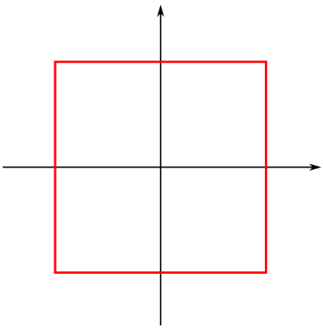
\includegraphics[scale=0.4]{figures/square.png}
	\caption{Apenas um quadrado. Fonte:\cite{jakob} }
\end{figure}
Podemos fazer uma rotação desse quadrado em torno desse plano de, digamos, $5^{\circ}$ no sentido horário. Nesse caso, o quadrado agora estaria da seguinte forma 
\begin{figure}[H]
	\centering
	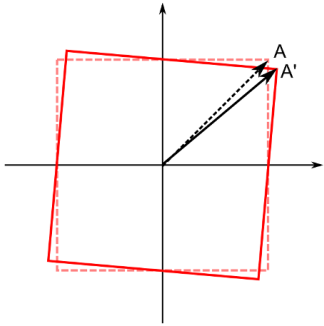
\includegraphics[scale=0.4]{figures/square5.png}
	\caption{Quadrado rotacionado de $5^{\circ}$. Fonte:\cite{jakob} }
\end{figure}
Veja que a transformação que aplicamos foi uma rotação. Porém, é notável que verificamos uma diferença nesse quadrado após essa rotação. Mas agora, se rotacionarmos esse quadrado em $90^{\circ}$, 
\begin{figure}[H]
	\centering
	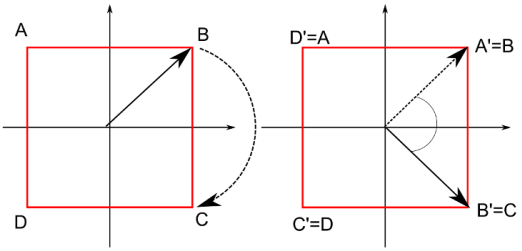
\includegraphics[scale=0.4]{figures/square90.png}
	\caption{Quadrado rotacionado de $90^{\circ}$. Fonte:\cite{jakob} }
\end{figure}
Verificamos que não é possível dizer se ele foi rotacionado ou não. Para entender melhor isso, suponha que você feche os olhos e então nós façamos essa rotação de $90^{\circ}$. Após você abrir os olhos novamente, você acreditaria que o quadrado está da mesma forma. Isso é o que chamamos de uma \textit{simetria}. 

Nesse caso, no entanto, essa simetria é caracterizada como uma simetria \textit{discreta}, pois não é qualquer rotação que deixa o quadrado invariante, mas sim rotações múltiplas de $90^{\circ}$. 

Outro exemplo que podemos usar é o do círculo. 
\begin{figure}[H]
	\centering
	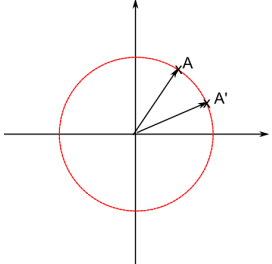
\includegraphics[scale=0.5]{figures/circ.png}
	\caption{Apenas um círculo. Fonte: \cite{jakob}}
\end{figure}
Nesse caso, é fácil perceber que qualquer rotação deixa o círculo invariante. Faça o mesmo experimento mental de fechar os olhos e então abri-los novamente. Independemente de qualquer rotação que façamos no círculos, você nunca será capaz de perceber se ele foi rotacionado ou não. 

Nesse caso, dizemos que é uma simetria \textit{contínua}, pois o círculo é simétrico para quaisquer ângulos de rotação. 

Isso nos permite concluir algumas coisas. 
\begin{itemize}
	\item Se compormos duas rotações, isto é, rodarmos de $20^{\circ}$ e depois rodarmos de $10^{\circ}$, isso equivale a uma rotação de $30^{\circ}$. Portanto, a composição de duas rotações também deve ser uma rotação. 
	\item Podemos não fazer nenhuma rotação, o que equivale a um ângulo de rotação de $0^{\circ}$. Isso é o que chamamos de um elemento \textit{identidade.} Portanto, uma identidade sempre é uma simetria e então deve ser levada em consideração quando estivermos falando dessa caoleção de transformações. 
	\item Nós tomamos uma rotação no sentido horário. Mas podemos muito bem tomar rotações no sentido anti-horário. Isso implica que se fizermos uma rotação de $45^{\circ}$ no sentido horário, podemos desafazê-la simplesmente rodando de $45^{\circ}$ no sentido anti-horário. Isso é o que chamamos de um elemento \textit{inverso.}
	\item Por último, rodar de $90^{\circ}$ seguida de uma rotação de $40^{\circ}$ seguida de uma rotação de $110^{\circ}$ deve ser equivalente a uma rotação de $130^{\circ}$ seguida de uma rotação de $110^{\circ}$, que deve ser equivalente a uma rotação de $90^{\circ}$ seguida de uma rotação de $150^{\circ}$. Dizemos então que as rotações são \textit{associativas.} Matematicamente esta ideia é representada por 
	$$
	R(110^{\circ})(R(40^{\circ})R(90^{\circ}))=R(110^{\circ})R(130^{\circ})=(R(110^{\circ})R(40^{\circ}))R(90^{\circ})=R(150^{\circ})R(90^{\circ})
	$$
\end{itemize}
Dadas essas ideias intuitivas, veremos agora como as generalizamos matematicamente.  
\subsection{Definição de grupo}
Um grupo é um conjunto $G$ com um mapa $\cdot$ que é chamado de \textit{regra de composição}, que satisfaz as seguintes propriedades:  
\begin{itemize}
	\item \textbf{Fechamento:} Para todo $g,g'\in G,\; g\cdot g'\in G.$ 
	\item \textbf{Identidade:} Existe um elemento $e\in G$ tal que para todo $g\in G$, $g\cdot e=e\cdot g = g$. Chamamos esse elemento de \textbf{identidade. }
	\item \textbf{Elemento inverso}: Para todo $g\in G$, existe $g'\in G$ tal que $g\cdot g'=g'\cdot g = e$. Chamamos esse elemento de\textbf{ inverso} e o denotamos por $g'\equiv g^{-1}$. 
	\item \textbf{Associatividade:} Para todo $g_1,g_2,g_3\in G,(g_1\cdot g_2)\cdot g_3=g_1\cdot(g_2\cdot g_3).$
\end{itemize}
Abaixo, vamos dar alguns exemplos de conjuntos simples que formam grupos, e como a regra de composição de dois elementos não precisa ser necessariamente uma multiplicação. 
\begin{example}[Números reais sobre multiplicação]
	O conjunto de números reais $\mathbb{R}$ forma um grupo sobre a multiplicação. 
	\begin{itemize}
		\item \textbf{Fechamento}: A multiplicação de dois números reais continua dando um número real. 
		\item  \textbf{Identidade}: O número 1 pode ser usado como uma identidade sobre a multiplicação. 
		\item \textbf{Elemento inverso:} Para todo número real $a$ a inversa desse número é simplesmente $1/a$, que também é um numero real, de forma que $a\cdot\frac{1}{a}=1$. 
		\item \textbf{Associatividade:} Segue facilmente da multiplicação de números reais.
	\end{itemize}
\end{example}
\begin{example}[Números inteiros sobre multiplicação]
O conjunto de números inteiros $\mathbb{Z}$ não forma um grupo sobre a multiplicação.

Isso segue facilmente quando consideramos o elemento inverso. Para os números reais, bastava inverter o número e teríamos o seu inverso. Porém, no caso dos inteiros, dado um inteiro $a$, o número $1/a$ não é inteiro. Portanto não existe um elemento inteiro que pode servir como inverso sobre a multiplicação.
\end{example}
\begin{example}[Números inteiros sobre a adição]
Tome o conjunto dos inteiros $\mathbb{Z}$ mas com a regra de composição sendo a adição $+$. 
\begin{itemize}
	\item \textbf{Fechamento:} A adição de dois números inteiros continuando sendo um número inteiro. 
	\item \textbf{Identidade:} A identidade, por definição é um elemento que não realiza nenhuma mudança quando composta com qualquer outro elemento do grupo. No caso da adição, esse elemento é o inteiro 0, pois 
	$$
	n+0=n, n\in\mathbb{Z}.
	$$
	\item \textbf{Elemento inverso:} No caso do elemento inverso, podemos usar um número negativo, isto é, 
	$$
	n+(-n)=0,n\in\mathbb{Z}.
	$$
	\item \textbf{Associatividade:} A associatividade segue trivialmente da soma dos números inteiros. 
\end{itemize}
\end{example}
Isso mostra que, de fato, a regra de composição nem sempre será uma multiplicação entre os elementos. 
\section{Rotações}
Esta seção será dedicada a compreensão de um grupo extremamente importante na física: o grupo de rotações. Começaremos discutindo o caso mais simples que são rotações no plano, e depois discutiremos como realizá-las de outra maneira, usando números complexos. Após isso, vamos falar sobre rotações em 3 dimensões e como realizá-las utilizando um ``análogo'' aos números complexos, porém em 4 dimensões, chamados de \textit{quaternions.}
\subsection{Rotações em duas dimensões}
A matriz de rotação em duas dimensões é representada\footnote{Memorize esse termo pois vai ser importante mais tarde.} por \textcolor{red}{(depois eu vou colocar a dedução dela aqui e tentar fazer na aula se der tempo)},
\begin{equation}\label{rotação 2d}
	R(\theta)=\begin{pmatrix}
		\cos\theta & -\sin\theta \\
		\sin\theta & \cos\theta 
	\end{pmatrix}.
\end{equation}
Essas transformações, como vimos nos exemplos iniciais, são transformações continuas, pois o ângulo de rotação $\theta$ pode variar continuamente no intervalo $\theta\in[0,2\pi)$. Em oposição, temos outros tipos de transformações, que não podem ser caracterizadas como rotações (vamos entender isso um pouco mais a frente), que são as \textit{reflexões}. Essas transformações são representadas matricialmente por
\begin{equation}
	P_x = \begin{pmatrix}
		-1 & 0 \\
		0 & 1
	\end{pmatrix},\quad 
	P_y= \begin{pmatrix}
		1 & 0 \\
		0 & -1
	\end{pmatrix},
\end{equation} em que $P_x$ é uma reflexão no eixo $x$ e $P_y$ é uma reflexão no eixo $y$. 
Diferentemente de uma rotação, essa transformação inverte apenas um dos eixos de uma forma que não é contínua. Dessa forma, reflexões são transformações discretas. 

Vamos verificar que de fato rotações formam um grupo. 
\begin{itemize}
	\item \textbf{Fechamento:} \begin{equation*}
		\begin{split}
	R(\theta)R(\theta')&= \begin{pmatrix}
		\cos\theta & -\sin\theta \\
		\sin\theta & \cos\theta 
	\end{pmatrix}\begin{pmatrix}
	\cos\theta' & -\sin\theta' \\
	\sin\theta' & \cos\theta' 
	\end{pmatrix}\\&=\begin{pmatrix}
	\cos\theta\cos\theta'-\sin\theta\sin\theta' & -\cos\theta\sin\theta'-\sin\theta\cos\theta' \\
	\cos\theta\sin\theta'+\sin\theta\cos\theta' & \cos\theta\cos\theta'-\sin\theta\sin\theta'
	\end{pmatrix}\\&=\begin{pmatrix}
	\cos(\theta+\theta') & -\sin(\theta+\theta') \\
	\sin(\theta+\theta') & \cos(\theta+\theta')
	\end{pmatrix}.
	\end{split}
\end{equation*}
Ou seja, a composição duas rotações é uma rotação com os ângulos somados.
\item \textbf{Identidade}: Considerando $\theta=0$, que equivale a não rodar, a matriz (\ref{rotação 2d}) se torna 
\begin{equation*}
	R(0)=\begin{pmatrix}
		1 & 0 \\
		0 & 1
	\end{pmatrix},
\end{equation*}
que é justamente a matriz identidade. 
\item \textbf{Elemento inverso:} Da composição de matriz, temos que se tomarmos $\theta'=-\theta$, obtemos a matriz identidade. Ou seja, existe uma inversa e é exatamente $R(-\theta)$. Isso também pode ser verificado usando os métodos de álgebra linear para encontrar inversar de matrizes. Nesse caso usamos apenas nossa intuição física. 
\item \textbf{Associatividade:} Nesse caso, precisamos fazer a multiplicação de três matrizes $R(\theta)R(\theta')R(\theta'')$ e verificar que multiplicar $R(\theta)R(\theta')$ e depois $R(\theta'')$ ou multiplicar $R(\theta')R(\theta'')$ e depois multiplicar $R(\theta)$ não importa. \textbf{Porém}, em geral, a ordem da multiplicação de dois elementos de um grupo pode importar. Isto é, $R(\theta)R(\theta')\neq R(\theta')R(\theta)$. Quando a ordem não importa, dizemos que os elementos comutam e portanto este grupo é \textit{abeliano}. No caso contrário, o grupo é \textit{não abeliano.} Rotações no plano formam um grupo abeliano. 
\end{itemize}
As rotações tem uma característica muito importante. Elas deixam o tamanho de vetores invariantes. Isto é, uma vez que rodamos um vetor, não consideramos que é o mesmo vetor de antes, pois o que caracteriza um vetor é seu módulo, direção e sentido. Nesse caso, sua direção e sentido mudaram, porém não o seu módulo. Vamos entender as implicações disso. 

O módulo de um vetor é calculado fazendo o produto interno desse vetor com ele mesmo. Podemos denotar o vetor após uma rotação por $\vec{v}'$. Logo, temos que 
\begin{equation}
	\vec{v}'=R\vec{v}.
\end{equation} 
Como o módulo desse vetor não muda, temos que 
\begin{equation}
	\vec{v}'\cdot \vec{v}'=\vec{v}\cdot \vec{v}.
\end{equation}
Matricialmente, o produto interno de dois vetores é multiplicar um vetor linha por um vetor coluna, o que é equivalente a seu transposto. Logo, de outra forma 
\begin{equation*}
\begin{split}
		&\vec{v}^T\cdot \vec{v}'=\vec{v}^T\cdot\vec{v}\\
		&(R\vec{v})^T(R\vec{v})=\vec{v}^T\vec{v}\\
		&\vec{v}^TR^TR\vec{v}=\vec{v}^T\vec{v},
\end{split}
\end{equation*}
ou seja, para o módulo um vetor permanecer invariante sobre rotações, isso implica na condição 
\begin{equation}\label{ortogonalidade}
	R^TR=\mathds{1},
\end{equation}
em que $\mathds{1}$ é a matriz identidade. Dizemos que essa é a condição de ortogonalidade é então as rotações formam o \textit{grupo ortogonal $O(2)$}, que é o grupo de todas matrizes $2\times2$ ortogonais. Porém, podemos verificar que as reflexões também são ortogonais. Se queremos exluir as reflexões e trabalhar com um grupo que envolve apenas as rotações, devemos trabalhar com um subgrupo de $O(2)$. Para isso, veja que, tomando o determinante de ambos lados da equação (\ref{ortogonalidade}), 
\begin{equation*}
	\begin{split}
		&\det(R^TR)=\det(1)=1\\
		&\det(R^TR)=\det (R^T)\det (R)=1\\
		&\det(R)^2=1\\
		&\det(R)=\pm 1.
	\end{split}
\end{equation*}
Ou seja, temos dois possíveis valores de determinantes para matrizes ortogonais, +1 e -1. A matrizes com determinante +1 são as rotações. Portanto, definimos o subgrupo de $O(2)$, $SO(2)$, em que $S$ significa ``special'' para denotar que essas matrizes tem determinante +1. Logo, as rotações satisfazem as seguintes propriedades
\begin{itemize}
	\item $R^TR=\mathds{1}$,
	\item $\det(R)=1$.
\end{itemize}
\subsection{Rotações com números complexos}
\subsection{Rotações em três dimensões}
\subsection{Rotações com quaternions}
\section{Álgebra de Lie}
\subsection{Geradores}
\subsubsection{Geradores do grupo SO(3)}
\subsubsection{Geradores do grupo SU(2)}
\section{Teoria de Representação}
\subsection{Representações do grupo SU(2)}
\section{Grupo de Lorentz}


\pagebreak
\nocite{*}
\bibliography{refs.bib}
\bibliographystyle{ieeetr}
\end{document}
